%----------------------------------------------------------------------------------------
%	PACKAGES AND OTHER DOCUMENT CONFIGURATIONS
%----------------------------------------------------------------------------------------

\documentclass[twoside,twocolumn]{article}

\usepackage{blindtext} % Package to generate dummy text throughout this template 

\usepackage[sc]{mathpazo} % Use the Palatino font
\usepackage[T1]{fontenc} % Use 8-bit encoding that has 256 glyphs
\linespread{1.15} % Line spacing - Palatino needs more space between lines
\usepackage{microtype} % Slightly tweak font spacing for aesthetics

\usepackage[english]{babel} % Language hyphenation and typographical rules

\usepackage[hmarginratio=1:1,top=32mm,columnsep=20pt]{geometry} % Document margins
\usepackage[hang, small,labelfont=bf,up,textfont=it,up]{caption} % Custom captions under/above floats in tables or figures
\usepackage{booktabs} % Horizontal rules in tables

\usepackage{graphicx}

\usepackage{lettrine} % The lettrine is the first enlarged letter at the beginning of the text

\usepackage{enumitem} % Customized lists
\setlist[itemize]{noitemsep} % Make itemize lists more compact

\usepackage{abstract} % Allows abstract customization
\renewcommand{\abstractnamefont}{\normalfont\bfseries} % Set the "Abstract" text to bold
\renewcommand{\abstracttextfont}{\normalfont\small\itshape} % Set the abstract itself to small italic text

\usepackage{titlesec} % Allows customization of titles
\renewcommand\thesection{\Roman{section}} % Roman numerals for the sections
\renewcommand\thesubsection{\roman{subsection}} % roman numerals for subsections
\titleformat{\section}[block]{\large\scshape\centering}{\thesection.}{1em}{} % Change the look of the section titles
\titleformat{\subsection}[block]{\large}{\thesubsection.}{1em}{} % Change the look of the section titles

\usepackage{fancyhdr} % Headers and footers
\pagestyle{fancy} % All pages have headers and footers
\fancyhead{} % Blank out the default header
\fancyfoot{} % Blank out the default footer
\fancyhead[C]{Running title $\bullet$ May 2016 $\bullet$ Vol. XXI, No. 1} % Custom header text
\fancyfoot[RO,LE]{\thepage} % Custom footer text

\usepackage{titling} % Customizing the title section

\usepackage{hyperref} % For hyperlinks in the PDF

%----------------------------------------------------------------------------------------
%	TITLE SECTION
%----------------------------------------------------------------------------------------

\setlength{\droptitle}{-4\baselineskip} % Move the title up

\pretitle{\begin{center}\Huge\bfseries} % Article title formatting
	\posttitle{\end{center}} % Article title closing formatting
\title{Wind Farm} % Article title
\author{%
	\textsc{Niels van Duijn, Jurriaan Govers, Luuk van Hagen}\\
	\textsc{Jochem Hoorneman, Max van Leeuwen}\\%\thanks{A thank you or further information} [1ex] % Your name
	\normalsize TU Delft \\ % Your institution
	\normalsize \href{mailto:j.a.govers@gmail.com}{j.a.govers@gmail.com} % Your email address
	%\and % Uncomment if 2 authors are required, duplicate these 4 lines if more
	%\textsc{Jane Smith}\thanks{Corresponding author} \\[1ex] % Second author's name
	%\normalsize University of Utah \\ % Second author's institution
	%\normalsize \href{mailto:jane@smith.com}{jane@smith.com} % Second author's email address
}
\date{\today} % Leave empty to omit a date
\renewcommand{\maketitlehookd}{%
	\begin{abstract}
		\noindent This will be the abstract of our paper. We will show how cool our research is and how important we are. Blabla Lorem impsum.
	\end{abstract}
}

%----------------------------------------------------------------------------------------

\begin{document}
	
	% Print the title
	\maketitle
	
	%----------------------------------------------------------------------------------------
	%	ARTICLE CONTENTS
	%----------------------------------------------------------------------------------------
	
	\section{Introduction}
	
	\lettrine[nindent=0em,lines=3]To minimize cost of wind energy and to efficiently use resource rich locations, wind farms are constructed, characterized by a large concentration of wind turbines. An inherent side effect of wind turbine however is a wake. When wind turbines are placed in close proximity of each other in a wind farm, a wake can have negative effects. A wake forms behind an upwind wind turbine and can have severe effects on the power production and loads of the downwind turbine.

With an increasing role of wind energy in Europe's energy production (nationale energieverkenning) it is important for wind farms to be able to meet the demands of the power grid (Tande ). Controlling the power output of a wind farm is essential because an overload of energy can decrease the stability of the power system (Tande). Currently, most wind farms operate based on 'greedy control', meaning that the individual turbines always try to deliver maximum power. This causes a problem when the power demand is low and the dependency on the wind energy is high, resulting in an overload of the power system. Active power control can solve this problem, by regulating the power output of a wind farm.

There are several methods of active power control in a wind farm, two of which will be discussed in this paper, that is, yaw control and axial induction control. Yaw control can be used as a method to reduce the power output of a single wind turbine and as a method to increase power output of a wind farm and reduce loads (beetje gekke zin)(verwijzing). A disadvantage of yawing is an increase of the load on the turbine, and thus reducing its lifespan (Zalkind, Kanev). In addition, yawing a turbine can deflect a wake. This can be used as a method to redirect a wake from a downwind turbine, this would reduce the loads and increase power output of the downwind turbine. However, under unfavorable conditions it can result in an asymmetrical overlap of the wake on the downwind turbine. This can significantly increase the loads of the downwind turbine (Wilson, Van Dijk, Bastankah). As yawing of the turbine and the deflection of a wake can cause additional loads on the turbines of a wind farm, a trade of must be made between active power control and loads minimization. Axial induction can control the power output by varying the axial induction factor. Loads that are introduced by axial induction will not be discussed in this paper. 

Previous studies have mainly focused on optimizing the power output, rather than controlling the power output (verwijzingen naar studies die dit hebben gedaan).  Other studies focus on power optimization, while also taking the loads into account, so that an optimum is found between the two (verwijzing naar wie dit heft gedaan). The use of axial induction in optimizing power control has been marginally studied(heb hier nog geen goede bron voor kunnen vinden). Active power control through a combination of yaw control and axial induction control while minimizing loads is still novel.

This paper will focus on the optimization of active power control and loads by means of yaw control and axial induction control. In addition, a method is developed so that on-site power control can be realized.

\begin{equation}
\label{eq:P}
P_i = \frac{1}{2}\rho A_i C_p(a_i, \gamma_i)U_i^3
\end{equation}
Where,
\begin{equation}
\label{eq:Cp}
C_p(a_i, \gamma_i) = 4a_i(1-a_i)^2\eta cos(\gamma_i)^{pP}
\end{equation}

Let D denote bla, m bla, blabla.The wake is simulated using

\begin{equation}
\label{eq:Dw}
D_{w,i,q}(x) = max\left( {D_i + 2k_em_{e,q}([x - X_i],0} \right)
\end{equation}

\begin{equation}
\label{eq:Uw}
U_{w,i}(x,y) = U_i\left( {1-2a_ic_i(x,y)} \right)
\end{equation}

\begin{equation}
\label{eq:c}
c_{i,q}(x) = \left[ \frac{D_i}{D_i + 2k_em_{U,q}(\gamma_i)[x - X_i]} \right]^2
\end{equation}

\begin{equation}
\label{eq:mU}
m_{U,q}(\gamma_i) =  \frac{M_{U,q}}{cos(a_U+b_U\gamma_i)}
\end{equation}

\begin{figure}
\label{fig:wake}
  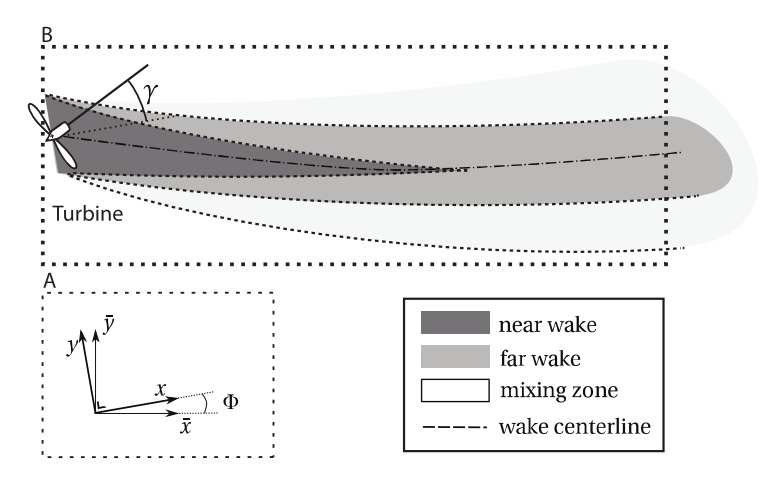
\includegraphics[width=\linewidth]{WakeFLORIS.png}
  \caption{A boat.}
  \label{fig:optim}
\end{figure}

The FLORIS model will be discussed in section \ref{sec:method}.
	
Hier nog een overzicht van wat er in paper te vinden is. Moet later geschreven worden als de rest af is.


	%------------------------------------------------
	
	\section{Method}
\label{sec:method}
	
	Short introduction on method 

%\noindent
	\textit{FLORIS}: The FLOw Redirection and Induction in Steady state (FLORIS) model gives a two-dimensional approximation of the steady-state effect of yaw misalignment and axial induction. It creates a wake model with equation (\ref{eq:c}  Wilson 3-3 tot 3-6). The wake is divided into three zones, $q_1$ to $q_3$, where $q_1$ refers to the near wake, $q_2$ to the far wake, and $q_3$ to the mixing zone (see Plaatje). FLORIS gives a power output for each turbine, which for turbine i results in equation (Wilson 3-1). Although less accurate than  SOFWA high fidelity CFD simulation, computation time is much faster for FLORIS. As a result, FLORIS can be used for on-site optimization. 



%\noindent
\textit{FAST \& MLife}: FAST (Fatigue, Aerodynamics, Structures and Turbulence) is a programming tool for the simulation of dynamic (load) responses of wind turbines (by NREL) (FAST documentatie). It uses wind turbine specifications as well as wind flow situations. By evaluating a flow field, FAST computes the bending moment of a blade. MLife is an application to process the bending moment to compute the damage equivalent loads (DELs). 



%\noindent
\textit{Inflow files, Flow field}: FLORIS describes a discrete flow field of a wake, with three zones. The flow field of the wake in FLORIS is calculated with equations (numbers). The wake is divided into three zones blab la as described in FLORIS-gedeelte. A real wake will not have discrete zones (Plaatje van dicrete wake), but a more fluent transition between the wake zones (Plaatje van de gaussian wake). To create a more fluent transition between the different wake-zones a Gaussian distribution of the flow field is preferred (Bastankah). The Gaussian distribution is calculated with equation (number), where the amplitude of the Gaussian, A, is equal to the velocity loss of the inner wake zone which is calculated with equation (number). Values $\sigma_y$ and $\sigma_z$, in equation (number), reflect the Gaussian standard deviation in horizontal and vertical direction, respectively. Both these standard deviations are linked to the spread of the Gaussian function. The standard deviations are linked to the outer wake zones, which are calculated by equations (numbers). In the model, $\sigma_y$ and $\sigma_z$ are a function of the diameter of the outer wake zone,  $D_{w,i,q=3}$, which is divided by a constant. This constant is equal to 4, which results in a standard deviation of two. As a result, the central 95.45\% of the values in the Gaussian distribution are taken. 
Wind shear can cause an important difference in velocity speeds between the rotor hub height, the end of the rotor blades at their highest points and the end of the rotor blades at their lowest point (Firtin). This velocity distribution is calculated with equation (number), where $v$ and $v_{ref}$ are the velocity at heights $h$, and $h_{ref}$  respectively. Value $\alpha$ is the wind shear coefficient which depends on different factors. Coefficient $\alpha$ is fixed at value 0.1, reflecting a terrain type close to ocean and smooth ground (Firtin). The wind shear is implemented in the flow field.


\begin{table}[h]
	%\renewcommand{\arraystretch}{1.3} 
	\caption{Overview of the minimum value, maximum value, and step size of the parameters diameter of outer wake zone (Dwake), freestream wind speed (U), yaw of the turbine (yaw), and the center to center distance between the center of the turbine and the center of the wake (y wake).}
	\centering
	\label{tab:pars}
	\begin{tabular}{lccc}
	\hline
	 & Minimum & Maximum & Step-size \\ 
	\hline
	Dwake & 180 & 330 & 25 \\
	U & -250 & 250 & 10 \\
	yaw & -30 & 30 & vary \\
	y wake & 2 & 8 & 2 \\
	\hline
	\end{tabular}

Note: Input values for yaw are [-30, -10, -5, 0, 5, 10, 30].
\end{table}

\begin{table}[h]
	%\renewcommand{\arraystretch}{1.3} 
	\caption{Overview of parametric parameters, with, the wake expansion factor for zone $i$ $m_{e,i}$, wake decay factor for zone $i$ $m_{U,i}$, wake decay parameters $a_U$ and $b_U$.}
	\centering
	\label{tab:pars}
	\begin{tabular}{ll}
	\hline
	Expansion & Velocity  \\ 
	\hline
	$k_d \qquad \quad 0.15$ & $M_{U,1} \quad 0.5$ \\
	$m_{e,1} \quad -0.5$ & $M_{U,2} \quad 1$ \\
	$m_{e,2} \qquad 0.22$ & $M_{U,3} \quad 5.5$ \\
	$m_{e,3} \qquad 1$ & $a_U \qquad 5$ \\
	& $b_U \qquad 1.66$ \\
	\hline
	\end{tabular}

Note: Table adjusted from Gebraad(nog correcte verwijzing toevoegen)
\end{table}

%\noindent
\textit{LUT}: To reduce computational time during optimization a look-up table (LUT) is created. The LUT is created using FAST and MLife, and it encompasses a wide variety of wind field conditions. 
These different conditions are described by the ranges of the parameters (see Table \ref{tab:pars}). The parameters are wake characteristics and can be extracted from FLORIS. The parameters chosen for the LUT are diameter of outer wake zone (Dwake), freestream wind speed (U), yaw of the turbine (yaw), and the center to center distance between the center of the turbine and the center of the wake (y wake).. The parameters are used to construct a flow field. Misschien nog een stukje over waarom deze parameters? Such that a four-dimensional LUT is created. The output of the LUT are the DELs. The LUT generation is time consuming, as such, it cannot account for all integer values of the parameters. The step-size of these parameters is chosen such that interpolation will give a representative result. For different parameters, different step-sizes are selected, as shown in Table (see Table \ref{tab:pars}). With the use of the pre-calculated LUT, the optimization can run more swiftly, and is able to be used on-site.

%\noindent
\textit{Optimization}: Game Theory
\begin{figure}
  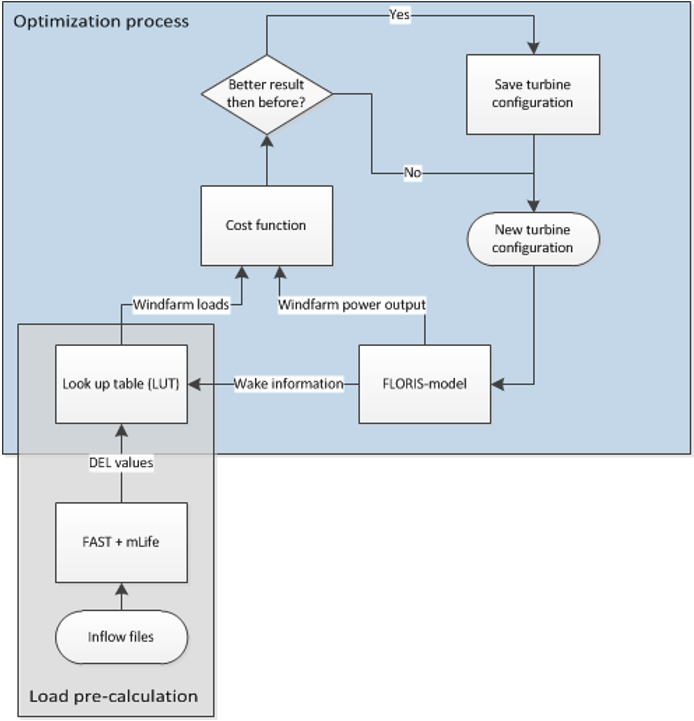
\includegraphics[width=\linewidth]{OptimizationProcess.png}
  \caption{A boat.}
  \label{fig:optim}
\end{figure}
	\begin{itemize}
		\item Here we introduce FLORIS, FAST, MLife
		\item FLORIS: why FLORIS compared to other software? How does FLORIS work? How do we use it?
		\item FAST \& Mlife:
		\item LUT: What is the LUT and why? What parameters did we choose, and why? Information about the step size of the parameters. Details in supporting info.
		\item Optimization: Game Theory
	\end{itemize}
	\blindtext % Dummy text
	





	Text requiring further explanation\footnote{Example footnote}.
	
	%------------------------------------------------
	
	\section{Results}
	
	Figures, tables with results and explanation.
	
	Discuss what can be improved
		
	\begin{table}
		\caption{Example table}
		\centering
		\begin{tabular}{llr}
			\toprule
			\multicolumn{2}{c}{Name} \\
			\cmidrule(r){1-2}
			First name & Last Name & Grade \\
			\midrule
			John & Doe & $7.5$ \\
			Richard & Miles & $2$ \\
			\bottomrule
		\end{tabular}
	\end{table}
	
	\blindtext % Dummy text
	
	\begin{equation}
		\label{eq:emc}
		e = mc^2
	\end{equation}
	
	\blindtext % Dummy text
	
	%------------------------------------------------
	
	\section{Discussion}
	
	\subsection{Subsection One}
	
	What have we done and how to interpret the results
	
	A statement requiring citation \cite{Figueredo:2009dg}.
	\blindtext % Dummy text
	
	\subsection{Subsection Two}
	
	Recommendations for further studies
	
	\blindtext % Dummy text
	
	%----------------------------------------------------------------------------------------
	%	REFERENCE LIST
	%----------------------------------------------------------------------------------------
	
	\begin{thebibliography}{99} % Bibliography - this is intentionally simple in this template
		
		\bibitem[Figueredo and Wolf, 2009]{Figueredo:2009dg}
		Figueredo, A.~J. and Wolf, P. S.~A. (2009).
		\newblock Assortative pairing and life history strategy - a cross-cultural
		study.
		\newblock {\em Human Nature}, 20:317--330.
		
	\end{thebibliography}
	
	%----------------------------------------------------------------------------------------
	
\end{document}
